\documentclass[11pt,a4paper]{article}
\usepackage[utf8]{inputenc}
\usepackage[T1]{fontenc}
\usepackage[spanish]{babel}
\usepackage{hyperref}
\usepackage{fontawesome5}
\usepackage[margin=1.55cm, top=1.2cm, bottom=1.3cm]{geometry}
\usepackage{titlesec}
\usepackage{enumitem}
\usepackage{setspace}
\usepackage{graphicx}

\hypersetup{
    colorlinks=true,
    linkcolor=black,
    urlcolor=blue,
}

\pagestyle{empty}
\setlength{\parindent}{0pt}
\setlength{\parskip}{0pt}
\setstretch{1.03}

\titleformat{\section}
    {\large\bfseries}
    {}
    {0em}
    {}
    [\vspace{-0.4em}\rule{\textwidth}{0.5pt}]

\titlespacing*{\section}{0pt}{1.2em}{0.7em}
\setlist[itemize]{leftmargin=1.15em, topsep=2pt, itemsep=3pt, parsep=0pt, label=\textbullet}

\begin{document}

\noindent
\begin{minipage}[c]{0.76\textwidth}
{\LARGE \textbf{JOAN MARQUEÑO SUREDA}}\\[0.2em]
{\normalsize Developer $\cdot$ Python $\cdot$ LLMs $\cdot$ Agentes $\cdot$ Kubernetes}\\[0.35em]
{\small
\faEnvelope\ \href{mailto:joan.marquenyo@gmail.com}{joan.marquenyo@gmail.com} $\cdot$
\faLinkedin\ \href{https://www.linkedin.com/in/joanmarqueno}{linkedin.com/in/joanmarqueno} $\cdot$
\faGithub\ \href{https://github.com/JoanMarqueno}{github.com/JoanMarqueno} $\cdot$
\faMapMarker\ Tarragona, España
}
\end{minipage}%
\hfill%
\begin{minipage}[c]{0.18\textwidth}
\raggedleft
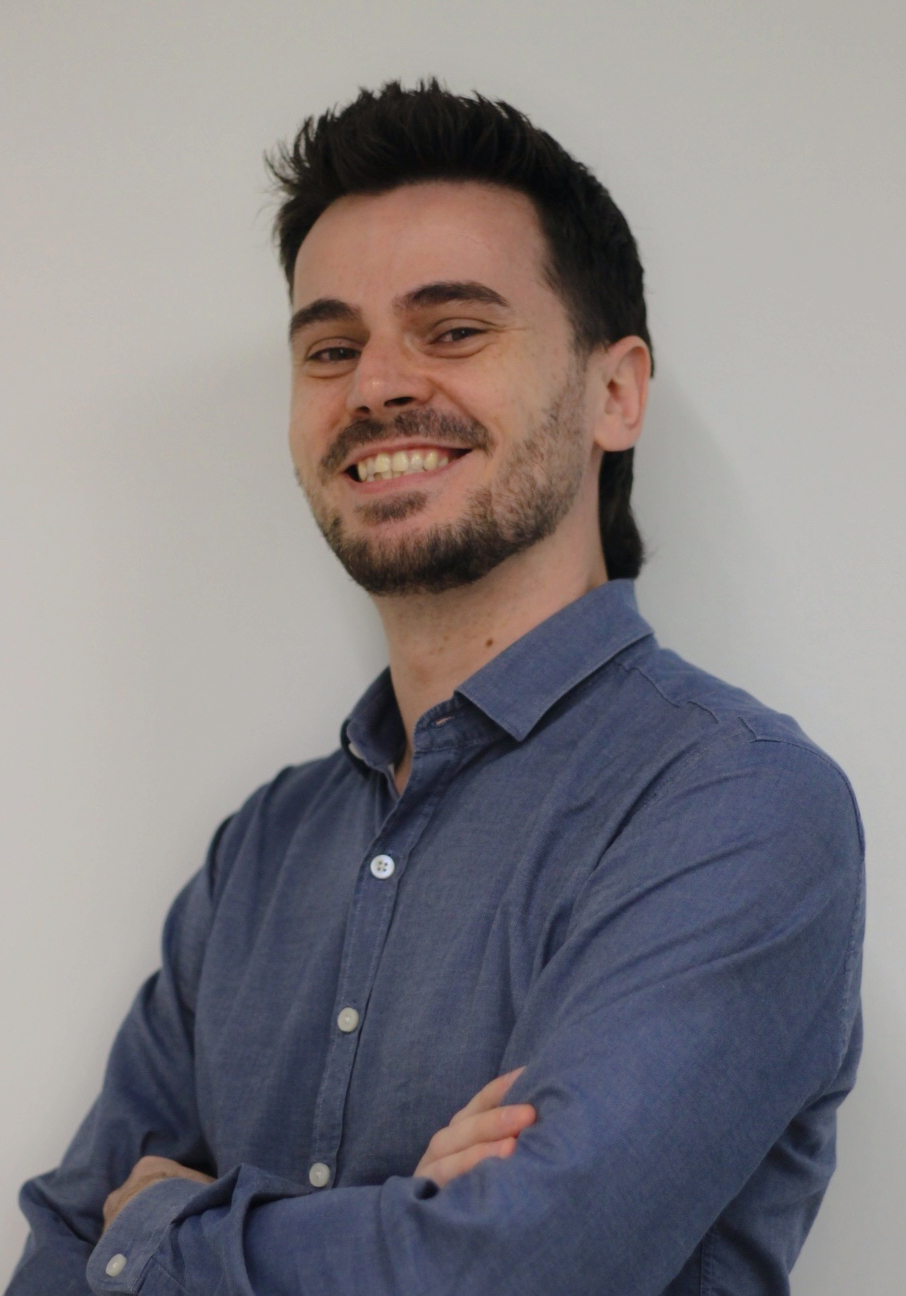
\includegraphics[width=2.35cm]{foto.jpg}
\end{minipage}

\vspace{0.55em}
{\footnotesize
\textbf{Python} $\cdot$ \textbf{TypeScript} $\cdot$ \textbf{LangChain} $\cdot$ \textbf{Azure OpenAI} $\cdot$ \textbf{RabbitMQ} $\cdot$ \textbf{Kubernetes} $\cdot$ \textbf{KEDA} $\cdot$ \textbf{Redis} $\cdot$ \textbf{PostgreSQL} $\cdot$ \textbf{pgvector} $\cdot$ \textbf{Docker} $\cdot$ \textbf{Azure} $\cdot$ \textbf{AWS} $\cdot$ \textbf{Hono} $\cdot$ \textbf{Next.js} $\cdot$ \textbf{Flutter}
}

\section*{RESUMEN PROFESIONAL}
Desarrollador especializado en \textbf{Python} y \textbf{sistemas LLM en producción}. \textbf{3+ años} construyendo una plataforma IDP enterprise con \textbf{+30 clientes activos}, \textbf{+1M de documentos procesados} y contratos de hasta \textbf{2M de documentos anuales}. Experiencia real en agentes con tool calling, orquestación event-driven, resolución de problemas de producción y arquitectura hexagonal en Kubernetes (Azure, AWS y on-premise).

\section*{EXPERIENCIA}

\textbf{Developer --- Python \& IA Aplicada} \hfill \textit{Jun 2023 -- Actualidad}\\[0.12em]
\textbf{INETUM} $\cdot$ Tarragona, España $\cdot$ \textit{Proyecto IIM-AI4CS}\\[0.15em]
\begin{itemize}
    \item Diseñé e implementé \textbf{+20 microservicios Python} especializados orquestados por un manager de flujos configurables y consumidos vía \textbf{RabbitMQ}: OCR, clasificación con Document Intelligence y LLM, extracción con GPT y tool calling, validación simple y cruzada, anonimización, transcripción multimedia con Whisper y conversión de formato.
    \item Agente GPT en producción con \textbf{tool calling} (crop de imagen, Bing Grounding vía LangChain) y \textbf{structured outputs} con strict mode y esquemas dinámicos por tipo documental; flujo \textbf{HITL} completo cuando las validaciones no superan el umbral de confianza.
    \item Resolví problemas reales de producción: token overflow por imágenes acumuladas en historial de agente, timeouts en lotes grandes, race conditions entre pods con distributed locking en \textbf{Redis}, y rate limits de Azure OpenAI con retry exponencial cogiendo el retry-after del header.
    \item Escalado automático con \textbf{KEDA} basado en profundidad de cola RabbitMQ, tenant isolation con colas y scalers dedicados por cliente, y observabilidad de costes de tokens por proyecto, modelo y servicio con dashboard propio y capping por variable de entorno.
    \item Plataforma desplegada en \textbf{Azure, AWS y on-premise} con arquitectura hexagonal, \textbf{Kubernetes}, \textbf{Keycloak} y configuración por cliente: \textbf{+30 clientes activos}, \textbf{+200.000 documentos/mes}, contratos de hasta \textbf{2M de documentos anuales}.
    \item \textbf{RAG} en MVP de gestión documental: chunking semántico con enriquecimiento de keywords y resumen, búsqueda vectorial con Azure AI Search y evaluación con golden datasets.
\end{itemize}

\vspace{0.5em}
\textbf{Assistant / Store / Multi Store Manager} \hfill \textit{Oct 2017 -- Ago 2022}\\[0.12em]
\textbf{PANDORA} $\cdot$ Barcelona / Tarragona, España\\[0.15em]
\begin{itemize}
    \item Liderazgo de equipos, KPIs y gestión operativa bajo presión --- experiencia hoy aplicada al trabajo con producto y negocio en proyectos de IA enterprise.
\end{itemize}

\section*{PROYECTOS PERSONALES}

\textbf{MysticMe} --- App móvil publicada en Google Play \hfill \textit{2023 -- Actualidad}\\[0.12em]
\begin{itemize}
    \item App de tarot y horóscopo desarrollada end-to-end de forma independiente. \textbf{Flutter} $\cdot$ \textbf{Dart} $\cdot$ \textbf{Supabase} $\cdot$ \textbf{Firebase Crashlytics}. Estrategia de crecimiento con TikTok/CapCut.
\end{itemize}

\vspace{0.45em}
\textbf{Kado Masajes} --- Web corporativa \hfill \textit{2024}\\[0.12em]
\begin{itemize}
    \item Web orientada a captación de contactos. \textbf{React} $\cdot$ \textbf{TypeScript} $\cdot$ \textbf{Tailwind CSS} $\cdot$ \textbf{Vite}.
\end{itemize}

\section*{FORMACIÓN \& CERTIFICACIONES}

\textbf{CFGS Desarrollo de Aplicaciones Multiplataforma} \hfill \textit{2022 -- 2024}\\[0.12em]
\textit{Institut Francesc Vidal i Barraquer} $\cdot$ Nota: \textbf{9,80} --- Matrícula de Honor\\[0.55em]
\textbf{Microsoft Certified: Azure AI Engineer Associate} \hfill \textit{Junio 2024}

\section*{SKILLS}
\textbf{IA \& Agentes:} LLMs, tool calling, structured outputs, HITL, visión multimodal, Whisper, LangChain, Azure OpenAI, Document Intelligence, RAG, pgvector.\\
\textbf{Backend:} Python, TypeScript, Hono, Zod, OpenAPI/Swagger, RabbitMQ, Redis, Peewee, Drizzle.\\
\textbf{Cloud \& Infra:} Kubernetes, KEDA, Azure, AWS, on-premise, Docker, Helm, Jenkins, Grafana, Keycloak.\\
\textbf{Frontend:} Next.js, React, Tailwind CSS, Flutter.\\
\textbf{Idiomas:} Español y catalán nativos $\cdot$ Inglés conversacional.

\end{document}
